\documentclass{beamer}

\usepackage[english]{babel}
\usepackage{xcolor}
\usepackage{xmpmulti}
\usepackage{amsmath}
\usepackage{dsfont}
\usepackage{multicol}
\usepackage{tikz}
\usepackage{eucal}
\usetikzlibrary{positioning,angles,quotes}
\usepackage{url}
\usepackage{graphicx}
\usepackage{cmbright}
\usepackage{framed}
\usepackage{tabularx}
\usepackage{amssymb}
\usepackage{pifont}

\usetikzlibrary{pgfplots.groupplots,arrows.meta,shadows,positioning,angles,quotes}
\usetikzlibrary{matrix,chains,positioning,decorations.pathreplacing,arrows}
\usepackage{tikz}
\usetikzlibrary{shapes.geometric}
\usetikzlibrary{positioning}
\usepackage{pgfplots}

%\input{epgfplotslibrary{groupplots}
\usetikzlibrary{pgfplots.groupplots,arrows.meta,shadows,positioning,angles,quotes}
\usetikzlibrary{matrix,chains,positioning,decorations.pathreplacing,arrows}

\newcommand{\xmark}{\ding{55}}

\DeclareMathOperator*{\argmax}{arg\,max}
\def\checkmark{\tikz\fill[scale=0.4](0,.35) -- (.25,0) -- (1,.7) -- (.25,.15) -- cycle;} 

\definecolor{Maroon}{cmyk}{0, 0.87, 0.68, 0.32}
\definecolor{RoyalBlue}{cmyk}{1, 0.50, 0, 0}
\definecolor{skymagenta}{rgb}{0.81, 0.44, 0.69}

\newenvironment{takeaway}[1]{%
	\definecolor{shadecolor}{gray}{0.9}%
		\begin{shaded}{\color{skymagenta}\noindent\textsc{#1}}\\%
		}{%
		\end{shaded}%
}



%%%%%% THE FOLLOWING FILE CONTAINS THE STYLE DEFINITIONS %%%%%%
\usepackage[utf8]{inputenc}
\usepackage[export]{adjustbox}

\definecolor{gris}{rgb}{0.92,0.92,0.92}
\definecolor{blau-upc}{rgb}{.192,.365,.506}

\setbeamercolor{titlelike}{fg=blau-upc}
% \setbeamercolor{barra}{bg=white,fg=white}
\setbeamercolor{capcalera}{bg=blau-upc,fg=white}
\setbeamercolor{section in toc}{fg=blau-upc}
\setbeamertemplate{sections/subsections in toc}[circle]
\setbeamertemplate{itemize items}[circle]
\setbeamercolor{item}{fg=blau-upc}
\setbeamertemplate{blocks}[rounded][shadow=true]
\setbeamercolor*{block body}{bg=gris}
\setbeamerfont{block body}{size=\footnotesize}
\setbeamercolor*{block title}{parent=structure,bg=blau-upc,fg=white}

\setbeamersize{text margin left=12mm,text margin right=12mm}
\setbeamertemplate{navigation symbols}{}

\setbeamertemplate{footline}[frame number]{}


\defbeamertemplate*{headline}{infolines theme}
{
	\begin{beamercolorbox}[wd=\paperwidth,ht=6.5mm,right]{white}%
		%\includegraphics[width = 45mm, height=10mm]{./logotips/visapp}\hspace*{2mm}\vskip0.2ex
	\end{beamercolorbox}
 	\begin{beamercolorbox}[wd=\paperwidth,ht=0.5mm,left]{barra}%
 		\hspace*{1mm}
 	\end{beamercolorbox}
}

\setbeamertemplate{footline}
{
	\hbox{
	\begin{beamercolorbox}[wd=0.1\paperwidth,ht=10mm,left]{}
% 		\hspace*{1ex}\includegraphics[height=8mm]{./logotips/imperiallogo.pdf}\vskip 2ex
	\end{beamercolorbox}
	\begin{beamercolorbox}[wd=0.8\paperwidth,ht=3ex,center]{}
		\hspace*{4ex}\insertsection\vskip 4ex
	\end{beamercolorbox}
	\begin{beamercolorbox}[wd=0.1\paperwidth,ht=3ex,right]{}
		\insertpagenumber\hspace*{6ex}\vskip 4ex
	\end{beamercolorbox}
	}
}

\setbeamertemplate{title page}
{
	\vbox{}
	\vfill
	\begin{centering}
		{\usebeamerfont{title}\usebeamercolor[fg]{title}\inserttitle}
		\vskip0.2em
		{\usebeamerfont{subtitle}\usebeamercolor[fg]{subtitle}\insertsubtitle}
		\vskip2em\par
		\small\insertauthor\par
		\vskip2em\par
		\tiny\insertdate\vskip1em\par
	\end{centering}
% 	\vfill
}

%\usebackgroundtemplate{\put(-50,-340){\includegraphics[width=10cm]{}}} 

%%%%%%

%%%%%% TITLE, AUTHOR, DATE DEFINITIONS %%%%%%
\title{Beyond Model-Free Reinforcement Learning}
	\subtitle{Solving Optimal Decision Making Problems from a Different Perspective}
\author{Matthia Sabatelli}

\date{\today}
%%%%%%

\setbeamertemplate{footline}[frame number]{}

\begin{document}

\frame{\titlepage} 

\begin{frame}{Recap}

	Last week we have seen ...
	\begin{block}{Model-Free Reinforcement Learning}
		\begin{itemize}
			\item How to construct algorithms when the state $|\mathcal{S}|$ and action spaces $|\mathcal{A}|$ are large
			\item Function Approximators
			\item Linear and Non-Linear Functions
			\item Deep Reinforcement Learning
			\item Experience Replay $D=\langle s_t, a_t, r_t, s_{t+1}\rangle$
		\end{itemize}
	\end{block}

\end{frame}



\frame{\frametitle{Today's Agenda}\tableofcontents}


\begin{frame}{Policy Gradient Methods}
	\section{Policy Gradient Methods}
	Throughout this course we have constantly seen how important \textcolor{RoyalBlue}{value functions} are:
	\begin{itemize}
		\item They correspond to the knowledge of the agent
		\item They help us understanding the environment
		\item But most importantly they define the policy $\pi$ that the agent follows
	\end{itemize}

	\bigskip

	$\Rightarrow$ The most \textcolor{skymagenta}{powerful} value function is the state-action value function $Q(s,a)$ since:
	\begin{align*}
		\pi^{*}(s) = \underset{a\in\mathcal{A}}{\argmax} \ Q^{*}(s,a) \ \text{for all} \ s \in \mathcal{S}
	\end{align*}

\end{frame}



\begin{frame}{Policy Gradient Methods}
	Our \textcolor{RoyalBlue}{goal} so far has always been that of learning $Q(s,a)$:
	\begin{enumerate}
		\item We can do this in a tabular fashion 
		\item Or we can generalize this process with a function approximator
		\item We can do this in an \textit{on-policy} or \textit{off-policy} fashion
	\end{enumerate}

	\bigskip

	$\Rightarrow$ \textcolor{RoyalBlue}{First} we learn a value function, and \textcolor{skymagenta}{then} we derive the policy $\pi$
	
	\bigskip
	
	$\Rightarrow$ We have \textcolor{Maroon}{never} seen how to learn $\pi$ directly!
	
\end{frame}


\begin{frame}{Policy Gradient Methods}
	Action value based methods such as Q-Learning, SARSA and $\text{QV}(\lambda)$ are very powerful algorithms but have some important \textcolor{Maroon}{limitations}:
	\begin{enumerate}
		\item Are restricted to discrete action spaces 
		\item Work alongside carefully designed exploration-exploitation strategies
		\item Are unable to learn an optimal policy which is stochastic 
		\item Sometimes learning $\pi(a|s;\theta)$ is easier than learning $Q(s,a;\theta)$
	\end{enumerate}

\end{frame}

\begin{frame}{Policy Gradient Methods}
	There is a family of techniques which tries to learn $\pi(a|s;\theta)$ directly:
	\begin{center}
		\textcolor{skymagenta}{\textbf{Policy Gradient Methods}}
	\end{center}

	\bigskip

	$\Rightarrow$ They learn a \textcolor{RoyalBlue}{parametrized policy} that learns how to select actions without having to consult a value function:
	\begin{align*}
		\pi(a|s;\theta)=\text{Pr}\:\{a_t = a, s_t=s\:;\theta_t=\theta\}
	\end{align*}

	\bigskip 

	The parameters $\theta$ usually correspond to the weights of a neural network

\end{frame}

\begin{frame}{Policy Gradient Methods}
	Training policy gradient methods significantly differs from training a Deep-Q Network:
	
	\bigskip

	$\Rightarrow$ The idea of last week's methods was that of \textcolor{Maroon}{minimizing} a certain quantity called the TD-error:
	\begin{align*}
		\mathcal{L}(\theta) = \mathds{E}_{\langle \cdot \rangle\sim U(D)} \bigg[\big(r_{t} + \gamma \: \underset{a\in \mathcal{A}}{\max}\: Q(s_{t+1}, a; \theta^{-}) - Q(s_{t}, a_{t}; \theta)\big)^{2}\bigg]
	\end{align*}

	
	\bigskip

	$\Rightarrow$ Policy Gradient methods instead seek to \textcolor{Maroon}{maximize} some scalar performance measure $J(\theta)$ and update the parameters via gradient ascent!
	\begin{align*}
		\theta_{t+1} = \theta + \alpha \widehat{\nabla J(\theta_t)}
	\end{align*}

\end{frame}


\begin{frame}{Policy Gradient Methods}
	It is also possible to learn $\pi(a|s;\theta)$ in \textcolor{RoyalBlue}{combination} with a value function!

	\bigskip

	$\Rightarrow$ These algorithms come with the name of \textcolor{skymagenta}{\textbf{Actor-Critic}} methods:
	\begin{itemize}
		\item It can be hard to learn a policy $\pi$ directly
		\item We would like to tell our agent learning who is learning $\pi$ how good its policy is 
		\item To do so we can use the state-value function $V^{\pi}(s)$
	\end{itemize}
\end{frame}


\begin{frame}{Policy Gradient Methods}
	How do Actor-Critic methods intuitively work?
		\begin{center}
			\begin{figure}
			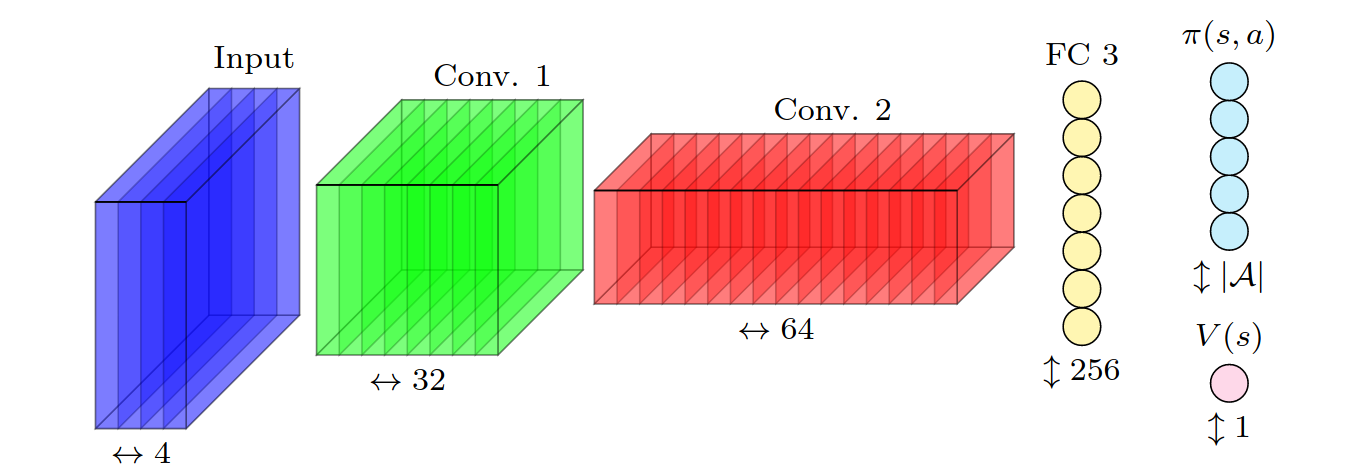
\includegraphics[width=\textwidth]{./Images/a2c}
			\caption{Image courtesy of Van de Wolfshaar (2017)}
			\end{figure}
		\end{center}
\end{frame}


\begin{frame}{Policy Gradient Methods}
	How do we train this network?

	\begin{align*}
		\theta_{t+1} & = \theta + \alpha \Big(r_t+\gamma V(s_{t+1};\phi)-V(s_t;\phi)\Big) \frac{\nabla\pi(a_t|s_t;\theta_t)}{\pi(a_t|s_t;\theta_t)} \\ 
			& = \theta_t + \alpha \delta_t \frac{\nabla\pi(a_t|s_t;\theta_t)}{\pi(a_t|s_t;\theta_t)} 
	\end{align*}

	\bigskip 

	$\Rightarrow$ Note that a value function ($\phi$) \textcolor{RoyalBlue}{helps} learning the policy parameters $\theta$ but is \textcolor{Maroon}{not required}
	for action selection purposes.
\end{frame}


\begin{frame}{Policy Gradient Methods}

	$\Rightarrow$ Nowadays actor-critic algorithms have become \textcolor{skymagenta}{very popular} in Deep Reinforcement Learning:
	\begin{enumerate}
		\item They are \textcolor{RoyalBlue}{theoretically motivated} thanks to the \textit{policy gradient theorem} (see page 325 of the book)
		\item The critic can technically learn \textcolor{RoyalBlue}{any value function}
		\item Can be massively parallelized (see A3C algorithm)
	\end{enumerate}

	\bigskip

	$\Rightarrow$ However, compared to action-value based methods, actor-critic algorithms are \textcolor{Maroon}{less well understood} (maybe because learning a policy $\pi$ is still more complex than learning a value function?) 

\end{frame}



\begin{frame}{Beyond Model-Free Learning}
	\section{Beyond Model-Free Learning}

	$\Rightarrow$ Actor-Critic algorithms, just like action value based methods are also \textcolor{RoyalBlue}{model-free} Reinforcement Learning algorithms.
	As a result we have never even attempted learning the transition function $\mathcal{P}$ of the Markov Decision Process $\mathcal{M}$.

	\bigskip

	\begin{itemize}
		\item Recall that the $\mathcal{P}$ and $\Re$ components of $\mathcal{M}$ are usually called the \textcolor{RoyalBlue}{model} of the environment
		\item If they are known we can use Dynamic Programming algorithms like \textcolor{RoyalBlue}{value iteration} :)
		\item However, in the typical Reinforcement Learning scenario this is \textcolor{Maroon}{never} the case :(
	\end{itemize}


\end{frame}


\begin{frame}{Beyond Model-Free Learning}
	What to do?

	\begin{itemize}
		\item In Model-Based Reinforcement Learning the goal is to \textcolor{RoyalBlue}{learn the model} of the environment through experience!
		\item The \textcolor{skymagenta}{idea} is to learn a function that comes in the following form: $f(s_t,a_t) = s_{t+1}$
		\item If learned $f$ would give us $p(s_{t+1}|s_t,a_t)$
		\item We can do somethinf similar for learning $p(r_t|a_t,s_t)$
	\end{itemize}
	
	\bigskip
	
	$\Rightarrow$ The task of learning a model of the environment corresponds to a \textcolor{RoyalBlue}{supervised learning} problem!

\end{frame}

\begin{frame}{Beyond Model-Free Learning}
	$\Rightarrow$ The overall learning strategy is very \textcolor{RoyalBlue}{simple}:
	
	\bigskip

	\begin{enumerate}
		\item We start with a random policy $\pi(a_t|s_t)$
		\item This policy results in a dataset of trajectories $\mathcal{D}=\{(s, a, s^{\prime})_i\}$
		\item We learn the dynamics of the model by minimizing $\sum_i ||f(s_i, a_i) - s_i^{\prime}||^{2}$
		\item Plan through the model and go back to step 2.
	\end{enumerate}

\end{frame}

\begin{frame}{Beyond Model-Free Learning}
	\begin{center}
		\begin{figure}
			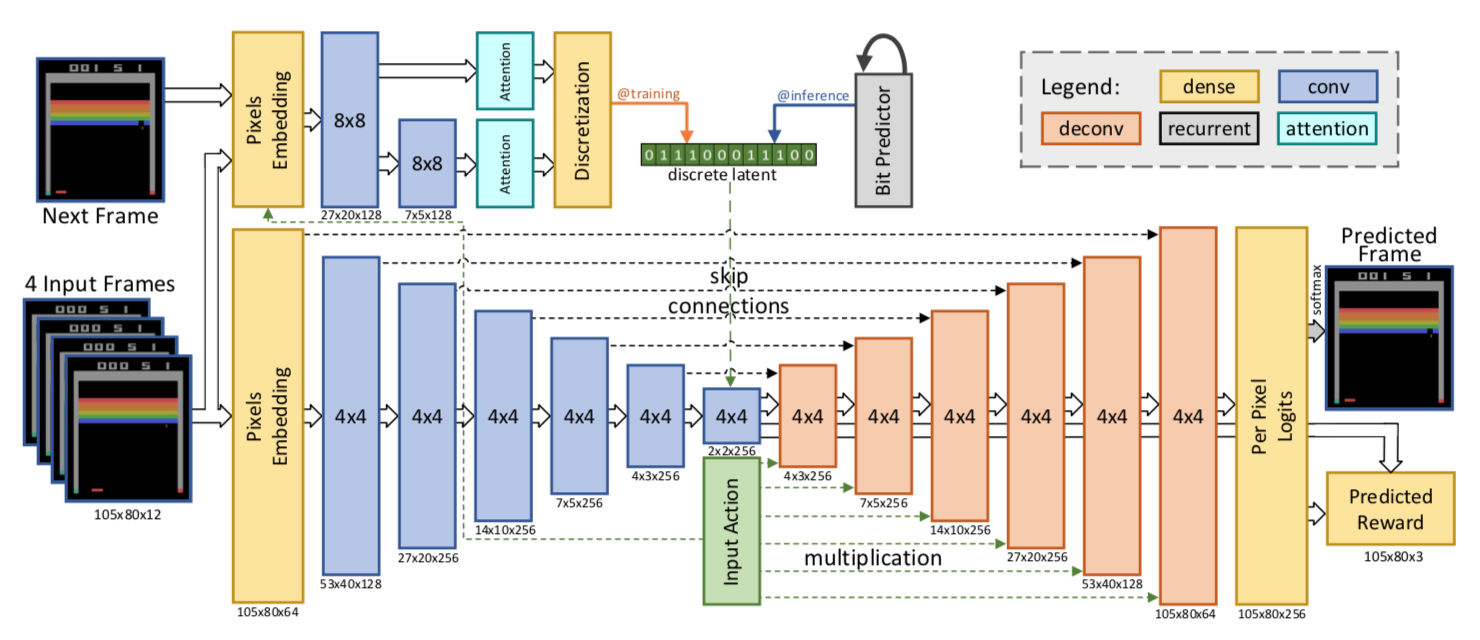
\includegraphics[width=\textwidth]{./Images/model_architecture}
			\caption{Image courtesy of Kaiser et al. (2020)}
			\end{figure}
	\end{center}
\end{frame}

\begin{frame}{Beyond Model-Free Learning}
	\begin{center}
		\begin{figure}
			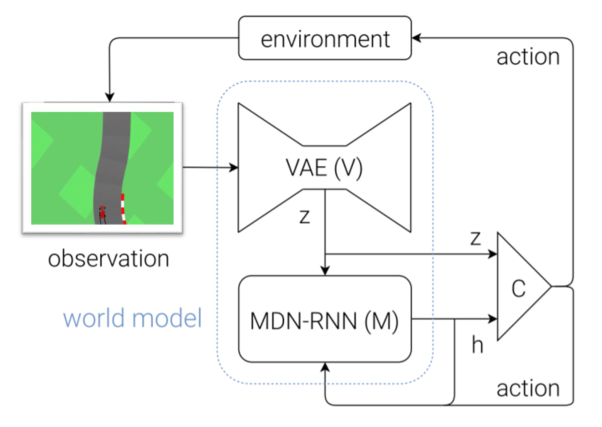
\includegraphics[width=9cm]{./Images/world_models}
			\caption{Image courtesy of Ha et al. (2019)}
			\end{figure}
	\end{center}
\end{frame}

\begin{frame}{Beyond Model-Free Learning}
	Pros \& Cons of Model-Based Reinforcement Learning:
	\begin{itemize}
		\item Some argue that learning $p(s_{t=1}|s_t,a_t)$ is easier than learning $Q^{\pi}(s,a)$ or $\pi(a|s)$ \textcolor{green}{\checkmark}
		\item If some dynamics of the environment are known it is easy to include them in the learning process \textcolor{green}{\checkmark}
		\item As it is essentially supervised learning it scales to a wide range of other applications (GANs and VAEs) \textcolor{green}{\checkmark}
		\item Is computationally very expensive \textcolor{red}{\xmark}
		\item What if the model is wrong? \textcolor{red}{\xmark}
	\end{itemize}
\end{frame}


\begin{frame}{Beyond Online Learning}
	\section{Beyond Online Learning}

	Throughout our lectures we have always assumed that the agent-environmnet interaction:
	\begin{enumerate}
		\item Can last as long as we want (possibly \textcolor{RoyalBlue}{infinite})
		\item Is \textcolor{RoyalBlue}{inexpensive}
		\item Moving from $s_{t}$ to $s_{t+1}$ is \textcolor{RoyalBlue}{fast}
		\item We have as many trajectories $\tau \langle s_t,a_t,r_t,s_{t+1}\rangle$ as we want at our disposal for learning
	\end{enumerate}

	\bigskip

	$\Rightarrow$ However, for many \textcolor{Maroon}{practical applications} this is not the case!

\end{frame}

\begin{frame}{Beyond Online Learning}
	Imagine the following situations:
	\begin{itemize}
		\item Clinical trials
		\item Self-driving cars
		\item Drones 
		\item Finance
	\end{itemize}

	\bigskip

	$\Rightarrow$ These are all examples for which it is \textcolor{Maroon}{very costly} to interact with the environment!

	We do have access to \textcolor{RoyalBlue}{some data} of the environment but not to the environment itself.
\end{frame}

\begin{frame}{Beyond Online Learning}
	Sometimes we have to train Reinforcement Learning algorithms with \textcolor{Maroon}{limited} data samples
	\bigskip
	
	\begin{center}
		\textcolor{skymagenta}{\textbf{Batch Reinforcement Learning}}
	\end{center}

	\bigskip

	$\Rightarrow$ We have a small dataset of trajectories $\tau \langle s_t, a_t, r_t, s_{t+1}\rangle$, collected by an unknown policy $\pi$ and wish
	to learn an \textcolor{RoyalBlue}{optimal value function}.

	\bigskip 

	The learning agent is \textcolor{Maroon}{not allowed} to gather any new experience!
\end{frame}


\begin{frame}{Beyond Online Learning}
	\begin{center}
		\begin{figure}
			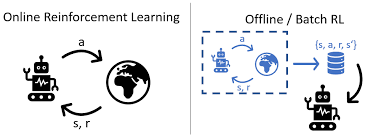
\includegraphics[width=9cm]{./Images/batch}
			\caption{Image courtesy of Swazinna et al. (2021)}
		\end{figure}
	\end{center}
\end{frame}

\begin{frame}{Beyond Online Learning}
	$\Rightarrow$ How do we \textcolor{RoyalBlue}{train} an agent in the Batch Reinforcement Learning context?
	
	\begin{enumerate}
		\item We start from a \textcolor{RoyalBlue}{dataset} $D$ of trajectories $\tau$ collected by policy $\pi^{\prime}$
		\item We train our favourite model-free algorithm on $D$ until \textcolor{RoyalBlue}{convergence}: $Q^{\pi^{\prime}}(s,a)$
		\item We can \textcolor{RoyalBlue}{deploy} the learned state-action value function to the environment and hope for the best
	\end{enumerate}

	\bigskip

	Where is the \textcolor{Maroon}{tricky} part?
	\begin{itemize}
		\item Our dataset of trajectories is very small \textcolor{red}{\xmark}
		\item Do you trust the $Q$ function that you have learned on $D$? \textcolor{red}{\xmark}
		\item We can only collect $D$ a few times \textcolor{red}{\xmark}
	\end{itemize}

\end{frame}

\begin{frame}{Beyond Online Learning}
	$\Rightarrow$ Batch Reinforcement Learning  poses some very interesting \textcolor{Maroon}{challenges} to the community:
	\begin{enumerate}
		\item It forces us to think in \textcolor{RoyalBlue}{practical terms}: we do not always have access to a simulation of the environment
		\item It questions the \textcolor{RoyalBlue}{reliability} of the mathematical tools we are using
		\item We need to reason about \textcolor{RoyalBlue}{uncertainty} even more: what if $D$ is only representative of a very small portion of $\mathcal{M}$
		\item Opens the door to \textcolor{RoyalBlue}{transfer-learning} training strategies
	\end{enumerate}

\end{frame}

\begin{frame}{Beyond Markov Decision Processes}
	\section{Beyond Markov Decision Processes}

	We have always modeled the \textcolor{RoyalBlue}{environment} as a Markov Decision Process:
	\begin{center}
		$\mathcal{M}\langle \mathcal{S}, \mathcal{A}, \mathcal{P}, r \rangle$
	\end{center}

	and assumed that the entire state space $\mathcal{S}$ is \textcolor{skymagenta}{visible} to the agent.

	\begin{center}
		\begin{figure}
			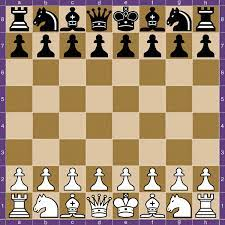
\includegraphics[width=4cm]{./Images/chess}
		\end{figure}
	\end{center}
\end{frame}

\begin{frame}{Beyond Markov Decision Processes}
	$\Rightarrow$ However there are many practical applications where it is \textcolor{Maroon}{impossible} for an agent to observe some states of the environment

	\begin{center}
		\begin{figure}
			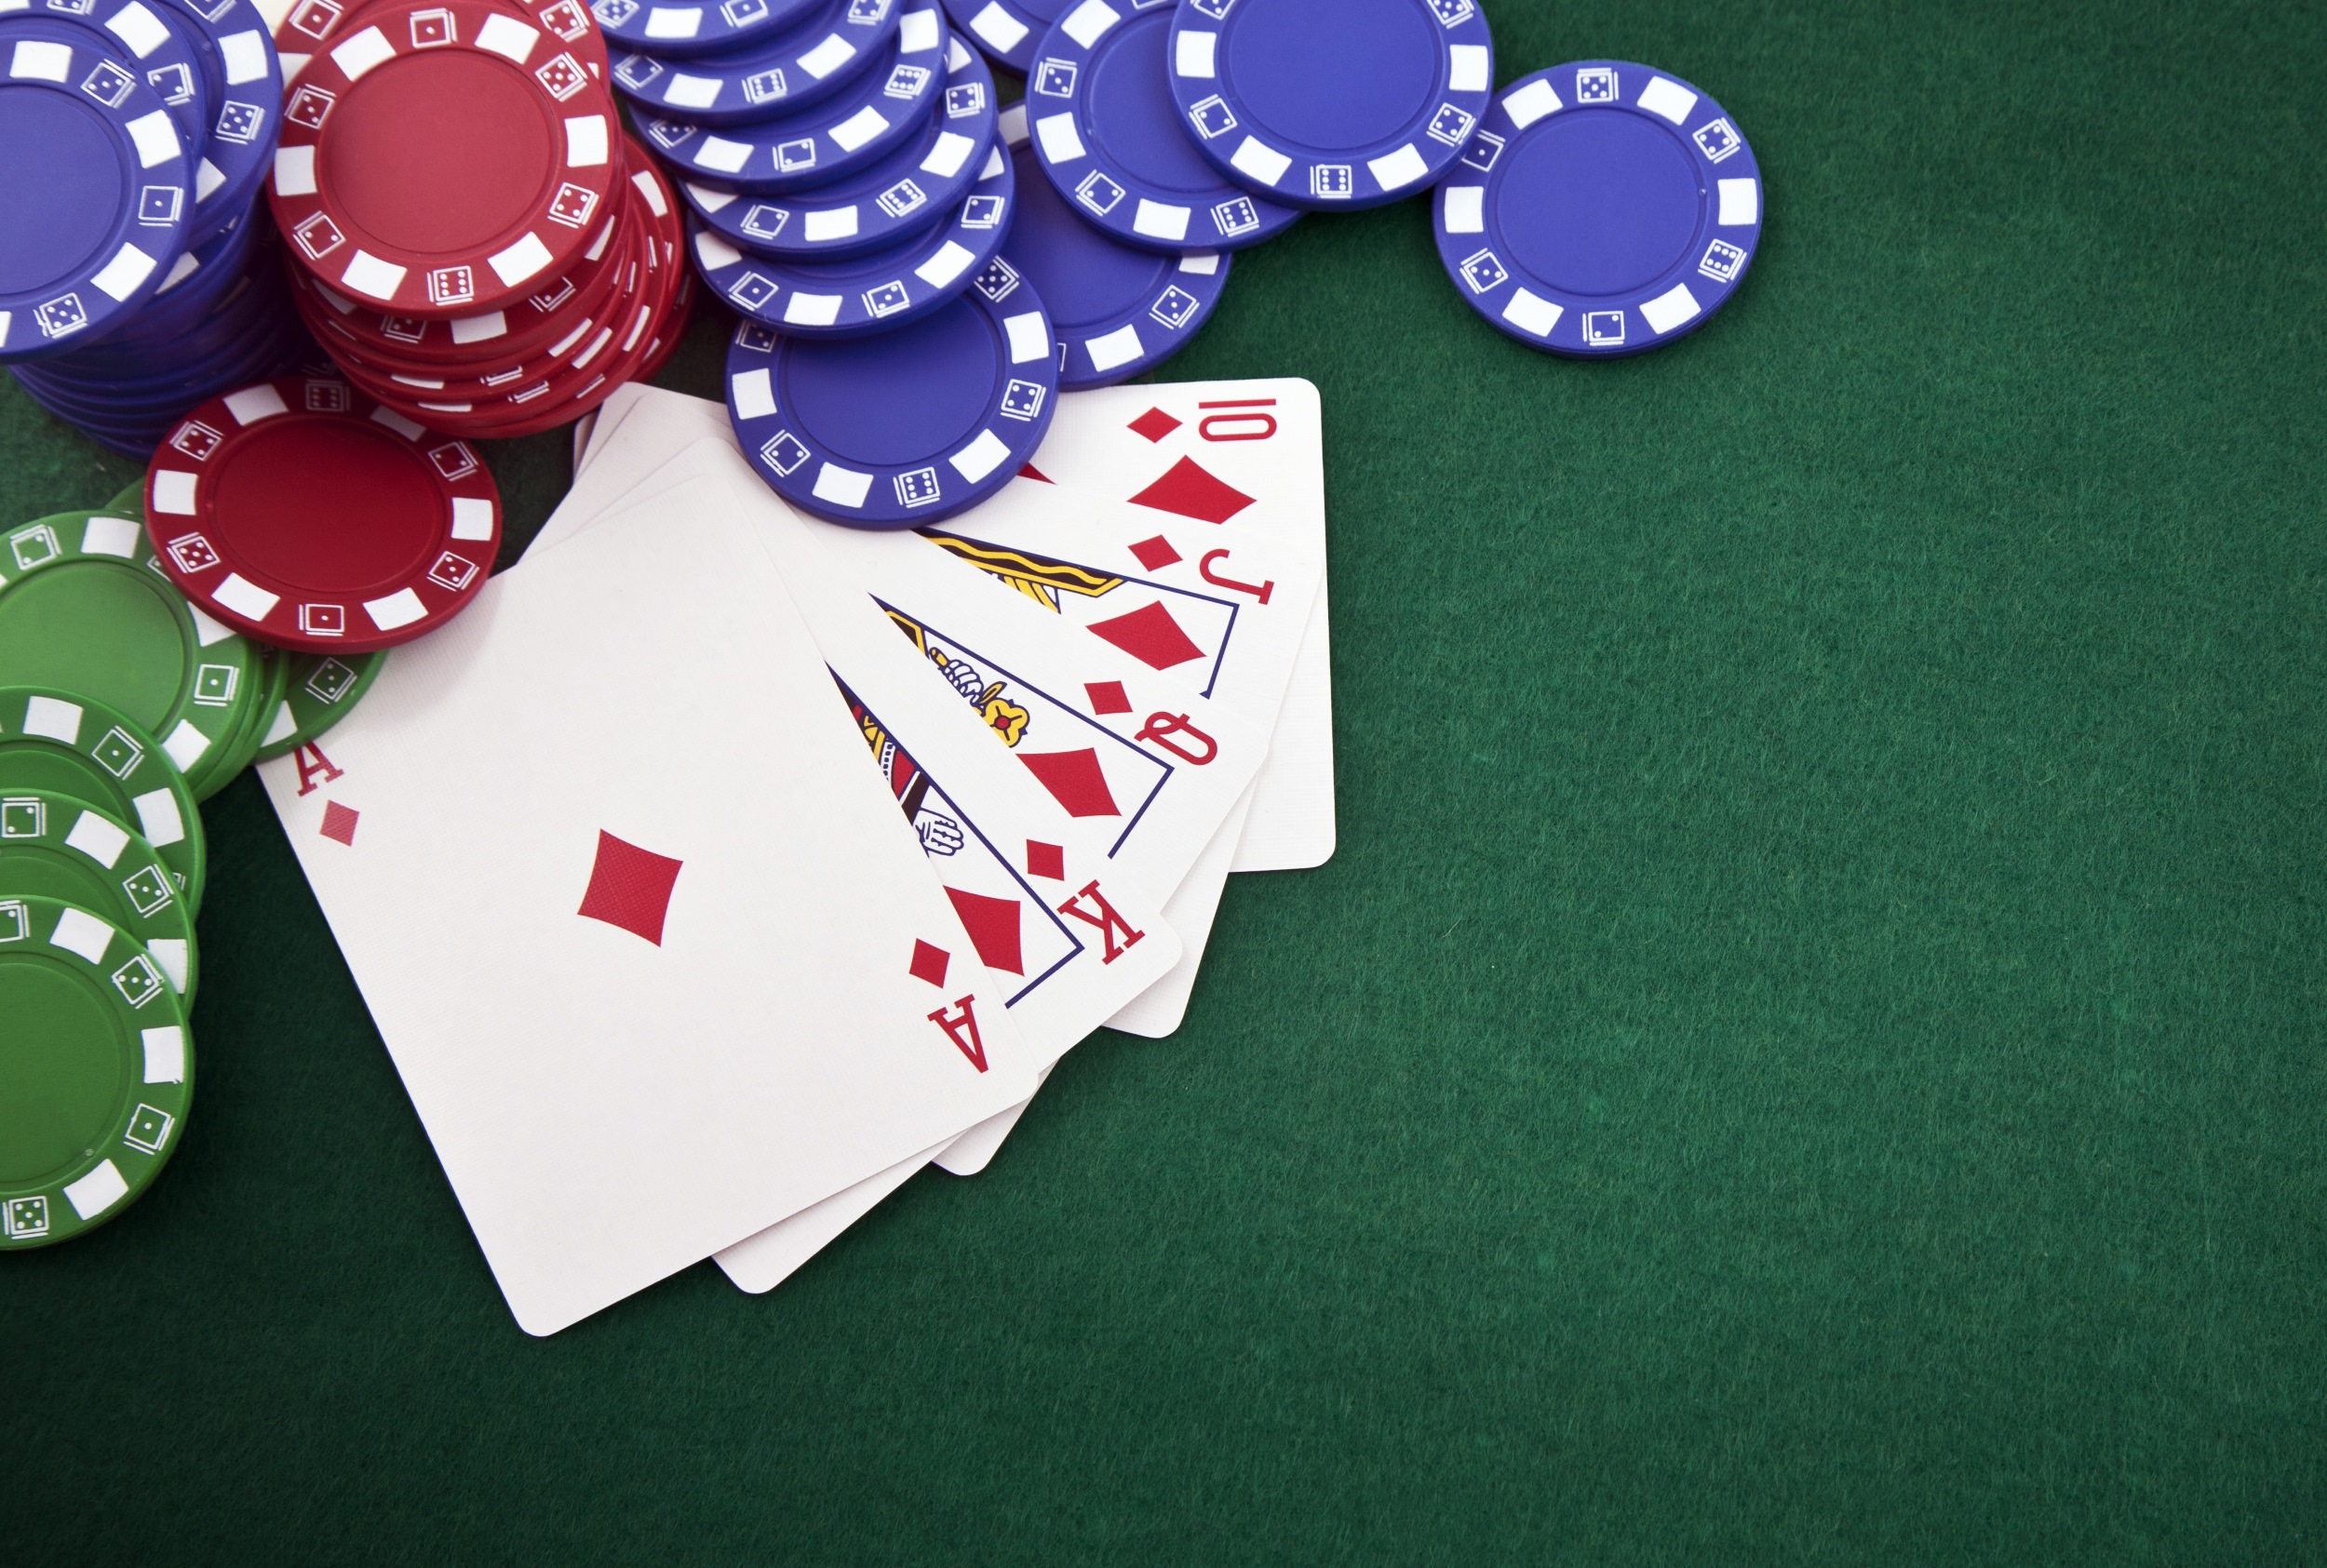
\includegraphics[width=5cm]{./Images/poker}
		\end{figure}
	\end{center}

	\bigskip

	How do we \textcolor{RoyalBlue}{formalize} such an environment?
\end{frame}

\begin{frame}{Beyond Markov Decision Processes}
	$\Rightarrow$ We \textcolor{skymagenta}{generalize} the concept of a MDP to a setting where once we have taken action $a_t$ we either can, or \textcolor{Maroon}{cannot} observe $s_{t+1}$: Partially Observable Markov Decision Process (POMDP)

	\begin{center}
		$\mathcal{M}\langle \mathcal{S}, \mathcal{A}, \mathcal{P}, r, \Omega, \mathcal{O}, \gamma \rangle$
	\end{center}

	%\bigskip

	We add two new components to the MDP:
	\begin{enumerate}
		\item $\Omega$ is a set of observations
		\item $\mathcal{O}$ are the conditional observation probabilities
	\end{enumerate}

	$\Omega$ gives us a \textcolor{RoyalBlue}{hint} about the state the agent is visiting, but not the true state itself!

\end{frame}

\begin{frame}{Beyond Markov Decision Processes}
	
	When dealing with a POMDP an agent deals with the \textcolor{RoyalBlue}{uncertainty} of the state space $\mathcal{S}$ by mantaining a \textcolor{RoyalBlue}{belief} $b$ over the visited states:
	\begin{itemize}
		\item $b$ represents a probabilty distribution $\mathcal{P}(\mathcal{S})$
		\item $b(s)$ denotes the probability $P(\mathcal{S}=s)$ under the current belief state
		\item Throughout interaction with the environment $b$ is updated
	\end{itemize}

	\bigskip

	$\Rightarrow$ The \textcolor{skymagenta}{goal} becomes to learn $\pi^{*}(b)$

\end{frame}

\begin{frame}
	\begin{center}
		\textcolor{skymagenta}{\textbf{The End !}}
	\end{center}
\end{frame}

\begin{frame}{In Memoriam: Marco A. Wiering (1971-2021)}
	\begin{center}
		\begin{figure}
			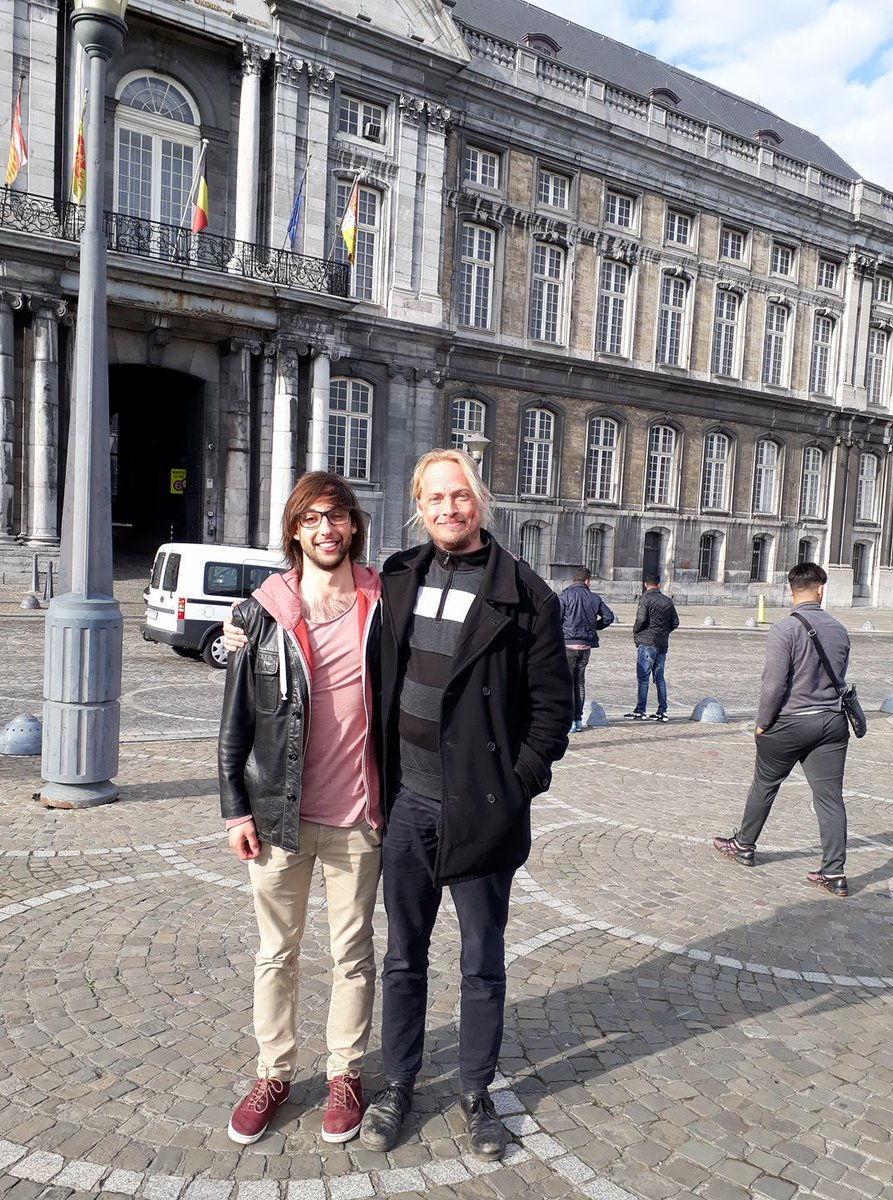
\includegraphics[width=5cm]{./Images/marco}
		\end{figure}
	\end{center}


\end{frame}




%============================================================================
\end{document}
